\documentclass{article}
\usepackage{fancyhdr}
\usepackage{tikz}
\usepackage{lipsum}
\usepackage{amssymb}
\usepackage{algorithm}
\usepackage{multirow}
\usepackage{subcaption}
\usepackage{pgfplots}

\usepackage{amsmath}
\usepackage{algorithmic}
\usepackage{array}

\usepackage[margin=1.5in]{geometry}
%\usepackage[pdftex]{graphicx}
\usetikzlibrary{positioning,automata, calc}


\graphicspath{{./images/}}
\DeclareGraphicsExtensions{.jpeg,.png,.jpg}
%\pagestyle{fancy}
%\lhead{Graph Theory}
%\chead{\today}
%\rhead{Andrew Felder}

\begin{document}
%\author{Andrew Felder}
%\title{Homework}
%\date{\today}
\begin{titlepage}
	\begin{center}
		\vspace*{1cm}
        
        \Large
        \textbf{Decentralized Hierarchical A* in a Multi-Agent System}
        
%        \vspace{0.5cm}
 %       Thesis Subtitle
        
        \vspace{1.5cm}
        \Large
        \textbf{Andrew Felder}
        
        \vfill
        
        A report presented for the final research\\
        of Graph Theory
        
        \vspace{0.8cm}
        
        
\includegraphics[width=0.4\textwidth]{UA_Logo}
        
        
        \Large
        Computer Science and Computer Engineering\\
        University of Arkansas\\
        \today
	\end{center}
\end{titlepage}
%\section{Abstract}
\begin{abstract}
This work addresses decentralized coordination of autonomous robots with assistance from overhead path planning cameras. I propose a solution that utilizes the performance of a decentralized system and handles dynamic environments in an efficient manner. Path planning was simulated in serial on various, randomized environments to show effectiveness. Path planning was then modified to operate in a multithreaded environment. This modification allowed for more realistic simulation of a multi-agent environment. This method efficiently handles the cases where other robot navigation methods are otherwise weak or ineffective.
\end{abstract}
\newpage
\tableofcontents
\newpage
\section{Introduction}
Indoor robot navigation has become a frequently researched area due to the increase of automation to augment jobs within warehouses and many other areas. This navigation is typically a combination of global planning and local planning, where the ground robots execute the results of the local plans. According to literature, \cite{PlanningSurveyParker}, one of the standards for robot navigation is to perform all planning on a central server which distributes instructions to each robot. From there, each robot will execute the path simultaneously since the central server calculates the paths relative to others in order to prevent deadlocks. The primary issue with this method is the single point of failure created by the central server.
Due to this, any downtime suffered by the central server limits or entirely halts all autonomous movement. 


In this work I show a system in which a hierarchical graph is used within a decentralized system to allow pathing in dynamic environments. This allows for the reduction of load on the robots that a centralized system provides while maintaining the efficiency of a decentralized system. By removing planning from the robots, it allows the robot to focus on supplemental tasks such as obstacle avoidance or cargo handling. Furthermore, as the regions are overseen by cameras, any environmental changes can be monitored and handled without requiring a robot to traverse the region. With this, robots can traverse only paths that are most optimal at all times. 


\section{Related Work}
To my knowledge, no work has been done in relation to a system of this type. Work has been done in decentralized multi-agent path planning. However, the standard for robot navigation is for the ground robots to calculate the paths themselves such as in \cite{DeadlockDigani}, \cite{DeadlockDraganjac}, \cite{FTC-A}, and \cite{DecentralizedPlanningVelagapudi}. Performing planning directly on the robots puts a heavy load on the robot and requires that they be equipped with unnecessarily powerful hardware. Further work has been done to reduce this load on the robots by employing hierarchical graphs which are used to perform path planning algorithms such as \cite{FTC-A} and \cite{CTF-A}. 

The previous work is primarily designed for a static environment. For dynamic environments, Simultaneous Localization and Mapping (SLAM) \cite{SLAM}, can be used. In this case, the robots are required to create the region's map locally. Unfortunately this means that before point-to-point planned navigation can take place, the area must be fully explored. While it is suited for dynamic environments, it is unaware of changes in the environment until the region is revisited by the robot. Further work has been done to allow this method to be both decentralized and distributed \cite{DecentralizedSLAM}.

For these multi-agent systems, work has also been done in avoiding deadlock. In \cite{DeadlockDigani}, the authors present a method based on resource allocation. This method requires robots to communicate as they approach an "intersection" to determine who the intersection is allocated to. In \cite{DeadlockDraganjac}, robots are given a "private zone" that is maintained as they navigate. If deadlock arises, one robot may move to a clear area in its private zone allowing the other robot to pass. In \cite{DecentralizedPlanningVelagapudi}, the authors make clever use of the birthday problem. A robot $r$ will share its path with a random set of robots $R_s$, a subset of all robots $R$. Each robot then builds a lookup table of its own path and those shared with it. Using this, there is a high probability that a pair of paths causing deadlock will be detected.
\section{Problem Statement}
Suppose there exists an arbitrary number of robots in a dynamic indoor environment. Also suppose there exists a series of decentralized cameras arranged in a grid layout with overlapping field of views between neighboring cameras. The objective is to dynamically and simultaneously provide guidance to all robots to safely reach their destinations.

\subsection{Assumptions}
For this work, it is assumed that the ground robots have Collision Detection capabilities, allowing them to stop if a collision were incoming. This potential collision could be with another robot or a person.

It is also assumed that a waypoint graph has been built in each region overseen by a camera such that any path covers clear ground exclusively. Methods for generating a waypoint graph have been discussed in \cite{WaypointJia} and \cite{WaypointVideoGames}.

\subsection{Definitions}

We define an environment for our system which resembles an industrial storage facility. This environment is dynamic and arbitrary. Our system consists of a set of ceiling-mounted smart cameras and a set of robots. 

A set of ceiling-mounted smart cameras view the entire working region of the environment, where an individual camera can see a small subset of the entire environment. Each camera has a working region which has slight overlap with all of its neighbors. These cameras are arranged in a grid in order to simplify this neighboring region overlap. The set of cameras are decentralized such that there is no central server performing any of the processing. For simplicity, each camera is mounted at the same height and each camera's region is the same size. At start-up, each camera performs an initialization phase which calculates a waypoint graph that represents its region.

Within the system, there exists a set of robots. After camera initialization, the robots received arbitrary instructions from a human user which tell the robot where to go (a goal which, in an industrial setting, would be where it would pick-up or drop-off cargo). The robots do not move synchronously. 

There exists middleware for communication between all agents in the system - camera-to-camera, robot-to-robot, robot-to-camera, and camera-to-robot. This communication is necessary for decentralization so that each agent can retrieve any information it requires.

% FIXME: need to better describe this image in this section FIXME %
\begin{figure}[!t]
\centering
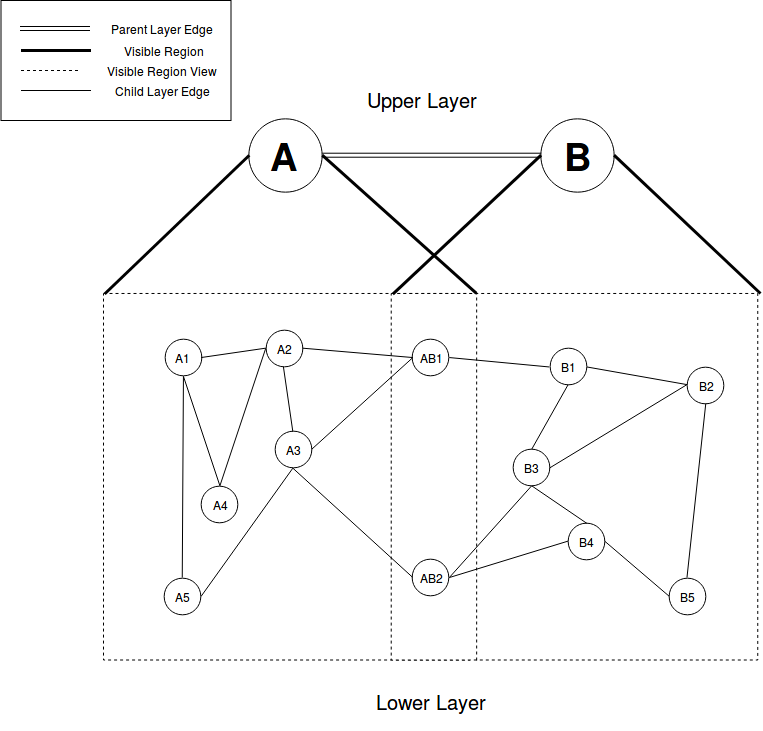
\includegraphics[width=3in]{HierarchicalSystem}
\caption{Simplified hierarchical network of nodes.}
\label{fig_hier}
\end{figure}

From here, we can decompose our system into a hierarchical graph where each region within a camera will be a set of child-layer nodes and each camera will be a parent-layer node. That is, each camera will be a parent to a set of nodes that exist within the waypoint graph of its region. Furthermore, each camera will have siblings that correspond to the neighboring cameras. This can be seen in figure \ref{fig_hier}. This figure shows a system containing two parent nodes, \{\(A,B\)\}. These nodes represent a ceiling-mounted smart camera in the physical system. Each of these parent nodes contains a set of child nodes, \{\(A1, A2, A3, A4, A5, AB1, AB2\)\} and \{\(B1, B2, B3, B4, B5, AB1, AB2\)\} respectively. Each child layer contains the points \{\(AB1, AB2\)\} which are therefore defined as overlap points as they are shared between parents.

We can define our upper-level system as an undirected graph, \(G = (V,E)\), where \(V\) is the set of cameras and where \(E\) defines the set of all edges that represent a pair of neighboring cameras. We further define our lower-level system as an undirected graph, \(G' = (V',E')\), where \(V'\) is the set of all waypoint nodes within each camera and where \(E'\) is the set of all edges that represent a pair of waypoint nodes. For each camera \(V_i\), there exists a set of child nodes \(C_i\).
We can declare a pair of cameras neighbors with the equation
\begin{equation}
\forall V_i, V_j \in V \ \exists E(V_i, V_j) \iff C_i \cap C_j \neq \varnothing
\end{equation}
Using this equation, it stands that neighbors have a set of overlapping points such that
\begin{equation}
O_{i,j} =  C_i \cap C_j
\end{equation} 
We then define a camera \(V_i\)'s unique set of child nodes to be 
\begin{equation}
P_i = C_i - \sum_j O_{i,j}
\end{equation}


We define our set of robots as \(R = \{ R_1, ..., R_k \}\) where the number of robots does not exceed \(V(G')\). The set of robots travel along the nodes of the lower-level graph, \(G'\). 

\subsection{Proposed Solution}
Current solutions to indoor robot navigation require a static environment in which calculations are performed by either a central server or the robots. In the case of robots performing calculations, each robots needs a local version of the entire map. If the environment is dynamic, it could be expensive to update the map of every robot. If the environment is dynamic, most solutions are ineffective or inefficient. 
I propose a solution that utilizes the performance of a decentralized system and handles dynamic environments in an efficient manner. 

This sytem uses an array of decentralized ceiling-mounted smart cameras covering the entirety of the map. Once the region is mapped, robots request a path from a source camera to a goal camera. Each camera may interact with with any other camera to incrementally build a path. Two version of A* were designed in this work. In the first, all processing is done on the source camera who will request information from any other camera in the system. In the second, the processing is done on the camera whose region is being checked. After it has finished the necessary processing, it will send required information back to the source camera. 

\section{Pathing}
To my knowledge, a method of path planning across a decentralized system we have defined does not exist. Similar work has been done for centralized systems in \cite{FTC-A} and \cite{CTF-A}. Therefore, we propose a modification to standard A*. As we don't have another method to compare against, we will use a greedy euclidean-based search as comparison. Since our system is intended to coordinate with other cameras within it, we are assuming that a camera in the upper layer has knowledge of other cameras' positions relative to itself. If this were not the case, we would be required to perform a blind search such as Uniform Cost Search. These cameras do not share any other knowledge.

\subsection{Greedy}
For the greedy method of path planning, we only take into account the euclidean distance between the current camera and the goal camera. Therefore nothing at the child level of the graph is considered. At each camera, we take the neighbor with the lowest euclidean distance to the goal camera and set it as the current camera. This would be equivalent to traversing a path through a camera in the direction of the goal, and replanning at each camera. This method runs until the goal is found. The path is rebuilt as described in Algorithm \ref{Rebuild_Path}

\subsection{A*}
I present two version of A* to solve the problem of decentralized pathing through this system. There are two primary changes made to the standard A* algorithm which are used in both versions. These changes are given in Algorithm \ref{D-A*_Cost} and \ref{Rebuild_Path}. Changes more specific to the two versions of D-A* will be presented in their section. 

\begin{algorithm}[h]
\caption{D-A* Cost}
\label{D-A*_Cost}
\begin{algorithmic}[1]
\REQUIRE \ \\
Current Camera, $C_C$ \\
Neighbor Camera, $C_N$ \\
\IF{$C_C$ is \textit{this}}
	\STATE Let $P_O$ represent a point in the overlap region between $C_C$ and $C_N$
	\RETURN path\_cost($C_C$.startPoint, $P_O$)
\ELSE
	\RETURN $C_C$.request\_cost($C_C$, $C_N$)
\ENDIF
\end{algorithmic}
\end{algorithm}

\begin{algorithm}[h]
\caption{Rebuild Path}
\label{Rebuild_Path}
\begin{algorithmic}[1]
\REQUIRE \ \\
Goal Camera, $C_G$ \\
Goal Point, $P_G$ in $C_G$ 
\STATE Let $C$ = $C_G$
\STATE Let $P_F$ be an initially empty set of edges representing the final path
\STATE Let $P_T$ be an initially empty set of edges representing an intermediate path
\WHILE{$C$.parent $\neq$ NULL}
	\STATE $P_T$ = \textit{this}.requestPath($C$.startPoint, $C$.endPoint)
	\STATE $P_T$.append($P_F$)
	\STATE $P_F$ = $P_T$
	\STATE $P_T$.clear()
\ENDWHILE
\end{algorithmic}
\end{algorithm}
\subsubsection{D-A* V1}
I propose Decentralized A* (D-A*), a modified version of A* to plan a path across a set of decentralized, connected parent nodes. The children of these nodes will be taken into account during the planning process. Work in decentralized path planning has been done in \cite{DecentralizedPlanningVelagapudi}, \cite{DeadlockDraganjac}. However, these algorithms run in a decentralized system where a robot or set of robots are self-sufficient. In this environment, I have a set of parent nodes creating a path through their children which the robots will follow. As it is decentralized, each parent node will have no knowledge of the internals of its neighbors. Therefore it will be necessary to use some form of network communication to request necessary information from other parent nodes.

This algorithm will follow a top down pathing approach. The majority of the pathing will happen on the parent layer with information such as cost coming from the child layer of the requested camera. The cost will be the shortest path across the child layer from the starting edge of the current camera to a point in the overlap region of the neighboring camera. For this algorithm, it is assumed that a pathing algorithm to determine the shortest paths on the child layer of every camera has already run. The primary difference between this and standard A* is the cost function and path rebuilding. This algorithm runs solely on the source camera which forces communication with other cameras for information. The path will be entirely rebuilt on the source camera, and passed along to the robot. Given all of this, I propose the following modifications to standard cost, path reconstruction, and A* algorithms in algorithms \ref{D-A*_Cost}, \ref{Rebuild_Path}, and \ref{D-A*} respectively. 

As this is a decentralized system, all method calls will be done on the source camera. Any calls that obtain information from a different camera will require a request to that camera. 

Per Algorithm \ref{D-A*_Cost}, if the source node is not the node we are seeking cost for, it will request cost from $C_C$ for a path from the start point of $C_C$ to a point in the overlap region shared with the neighbor in question. The cost of the path currently consists only of the length. Ideally, this could be expanded to include congestion at a time \(t\)

After the goal is found, the path will be rebuilt starting from the goal camera as described in Algorithm \ref{Rebuild_Path}. The source camera will request the path between the start and end points from the goal camera, and append it to the final path. The interior of the loop concatenates the most recently requested path onto the front of the final path. 

%Since we are operating on a standard grid, the currently used heuristic is Eucledian distance. However, as this is a modification to standard A*, the heuristic can be changed to fit the situation. 

The final modification to A* is on line 15 in algorithm \ref{D-A*}. As the cost in this implementation depends on the parent node, we check the cost of the path to reach the goal. Assume a goal camera, $C_G$ has two neighbors, $N_1$ and $N_2$. If $cost(N_1, C_G) < cost(N_2, C_G)$, then A* will assign $N_1$ as the parent of $C_G$.  Assume $O_{P1}$ is the overlap point between neighbor 1 and the goal. Assume $O_{P2}$ is the overlap point between neighbor 2 and the goal. Due to cost being directionally dependent, this could cause a problem when finding the path from the start point of $C_G$ to the goal point. This is because it is possible that $$pathCost(O_{P2}, goalPoint) < pathCost(O_{P1}, goalPoint)$$ If the difference is large enough, it may be true that the cost required to get to to the goal point would be lower if we followed the path along $N_2$.
\begin{align*}
	cost(N_1, C_G) &+ pathCost(O_{P1}, C_G.endpoint) \\
	&> \\
	cost(N_2, C_G) &+ pathCost(O_{P2}, C_G.endpoint)
\end{align*}
This would mean the path going through $N_1$ is suboptimal. Therefore we must take the extra path cost into account when assigning a parent to the goal node. This issue extends in that it could happen to any node farther than two steps from $C_S$. This causes A* to rarely produce a path which is longer than the path produced by greedy. In the case of the goal node, it is easily solvable. In the case of a random node, I believe this problem is not worth solving as it becomes very complex. I will discuss this in more detail in Sections 4.3 and 6.1.2.


\begin{algorithm}
\caption{D-A*}
\label{D-A*}
\begin{algorithmic}[1]
\REQUIRE \ \\
Start Camera, $C_s$ \\
Goal Camera, $C_g$ \\
Start Point $P_s$ in $C_s$
\STATE add $C_s$ to \textit{openSet}
\WHILE{\textit{openSet} is not empty}
	\STATE \textit{$N_C$} = \textit{openSet.pop}
	\IF{\textit{$N_C$} is $C_g$}
		\RETURN $C_S$.rebuild\_path()
	\ENDIF
	\FOR{each \textit{neighbor} of \textit{$N_C$}}
		\IF{\textit{neighbor} in \textit{closedSet}}
			\STATE \textbf{continue}
		\ENDIF
		\IF{\textit{neighbor} not in \textit{openSet}}
			\STATE add \textit{neighbor} to \textit{openSet}
		\ENDIF
		\STATE \textit{potentialCost} $=$ \textit{$N_C$}.costSoFar + $C_S$.cost(\textit{$N_C$, neighbor})
		\IF{\textit{neighbor} is $C_G$}
			\STATE \textit{ov\_point} $=$ find\_overlap\_point($N_C$, $C_g$
			\STATE \textit{potentialCost} $=$ $C_S$.getPathCost($C_G$.startPoint, $C_G$.endPoint)
		\ENDIF
		\IF{\textit{potential\_cost} $<$ \textit{neighbor}.costSoFar}
			\STATE $N_C$.endPoint $=$ find\_overlap\_point($N_C$, neighbor)
			\STATE \textit{neighbor}.startPoint = $N_C$.endPoint
			\STATE \textit{neighbor}.parent $=$ \textit{$N_C$}
			\STATE \textit{neighbor}.costSoFar $=$ \textit{potentialCost}
			\STATE \textit{neighbor}.costToEnd $\leftarrow$ \textit{neighbor}.costSoFar + heuristic()
		\ENDIF		 
	\ENDFOR
	\STATE \textit{closedSet}.add(\textit{$N_C$})
	\STATE \textit{openSet}.remove(\textit{$N_C$})
\ENDWHILE
\RETURN failure
\end{algorithmic}
\end{algorithm}
\subsubsection{D-A* V2}
This version of D-A* is modified such that the number of requests made on the network will be reduced. In the first version, only one set of information is gained per request. Assume a source node $C_S$ and a node currently being expanded, $C_C$. Since all processing is done in $C_S$, any time information is required from $C_C$, a request must be made. Due to the way A* works, only one neighbor of $C_C$ is processed at a time. Therefore, as we need information, such as cost, about each neighbor of $C_C$, a request must be made for each neighbor. As at least one neighbor of $C_C$ has already been discovered and expanded at this point, we have a maximum of 3 requests made to the same node. 

The goal of this version of D-A* is to reduce the number of requests made to $C_C$ by doing all neighbor processing on $C_C$ and returning the gathered information back to $C_S$. This gives us a maximum of 1 request to $C_C$ as illustrated in Figure \ref{fig:ReqDiagrams}. As these requests are only part of the total requests made, we will not achieve a 66\% decrease in total requests.

To do this, the calculations and evaluations for each neighbor must be moved into a function separate from D-A*. By moving lines 14-25 of Algorithm \ref{D-A*} into a separate function, \textit{getNeighborInfo()}, we can make a request on $C_C$ to run this function and return the information back. Given that, I propose the required modification to the neighbor loop in Algorithm \ref{V2Neighbor}. The evaluation of which set owns the neighbor is still required to be outside \textit{getNeighborInfo()} as we only want information on neighbors outside the closed set.

This modification was successful in greatly reducing the number of requests made across the network. This will be discussed more in the results section. 

\begin{algorithm}
\caption{D-A* V2 Neighbor Loop}
\label{V2Neighbor}
\begin{algorithmic}[1]
\STATE let \textit{neighbors} be an initially empty list
\FOR{each \textit{neighbor} of \textit{$N_C$}}
	\IF{\textit{neighbor} in \textit{closedSet}}
		\STATE \textbf{continue}
	\ENDIF
	\IF{\textit{neighbor} not in \textit{openSet}}
		\STATE add \textit{neighbor} to \textit{openSet}
	\ENDIF
	\STATE add \textit{neighbor} to \textit{neighbors}
\ENDFOR		 
\STATE $C_S$.getNeighborInfo(\textit{neighbors}, $N_C$, $C_G$)
\end{algorithmic}
\end{algorithm}

\begin{figure}[h]
\centering
\begin{subfigure}{.49\textwidth}
\centering
	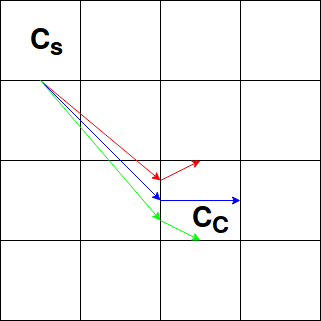
\includegraphics[width=.4\linewidth]{RequestDiagramV1}
	\caption{V1}
	\label{fig:v1Req}
\end{subfigure}
\begin{subfigure}{.49\textwidth}
	\centering
	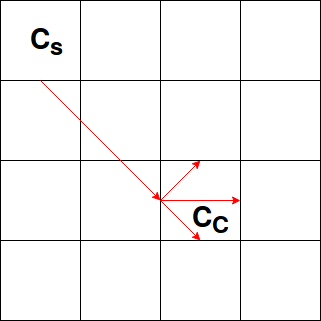
\includegraphics[width=.4\linewidth]{RequestDiagramV2}
	\caption{V2}
	\label{fig:v2Req}
\end{subfigure}
\caption{A visual representation of $C_S$ requesting information on $C_C$'s neighbors using D-A* V1 (a) and V2 (b). Each arrow from $C_S$ to $C_C$ represents a request on $C_C$ followed by which neighbor the request gathers information from.}
\label{fig:ReqDiagrams}
\end{figure}
\subsection{Lookahead Problem}
As described in section 4.2.1, pathing through this system is directionally dependant. This leads to issues in that the chosen path may not be the true optimal path. Because of this, a greedy search will outperform A* 2.42\% of the time. In this section, I will explain why this happens, but the percentage will be explained in results. 

This problem can be solved using a different representation of the system graph. However, without using a different representation, I believe it is not feasibly solvable. 

The graph representation used in this work is not a true representation of the graph. In this work, the graph is being represented as a grid of NxN nodes. The problem with this representation is that it assumes we are pathing from node center to node center, whereas we're actually pathing from node edge to node edge. Therefore, a more true representation would require treating each edge of each ceiling camera as a node or set of nodes as shown in Figure \ref{fig:RepDiagrams}. Using this representation would allow correct handling of directional dependency such that A* always outperforms greedy. However, this also means the potential size of the queue will be much larger, requiring more memory, and A* would take much longer to run.

\begin{figure}[h]
\centering
\begin{subfigure}{.49\textwidth}
\centering
	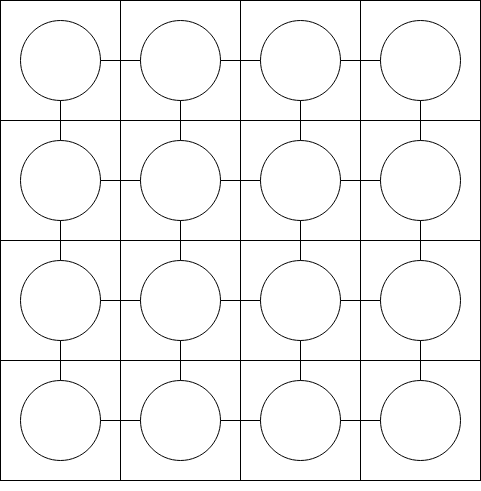
\includegraphics[width=.4\linewidth]{CurrentRepresentation}
	\caption{Current Representation}
	\label{fig:CurRep}
\end{subfigure}
\begin{subfigure}{.49\textwidth}
	\centering
	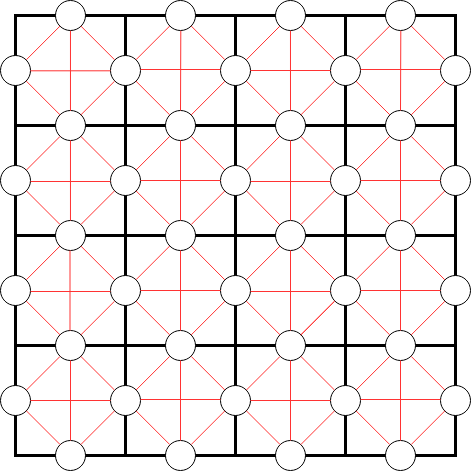
\includegraphics[width=.4\linewidth]{TrueRepresentation}
	\caption{"True" Representation}
	\label{fig:TrueRep}
\end{subfigure}
\caption{The currently used reprsentation (a) and the "True" representation (b). Note that both representations assume all nodes in the parent layer are connected to their neighbors. (b) assumes each edge can be reached by every other edge and that there is only one overlap point per edge.}
\label{fig:RepDiagrams}
\end{figure}

Using the current representation, the worst case Space Complexity is $\mathcal{O}(N^2)$. In the true representation, there are $N+1$ sets of $N$ nodes both from top to bottom and left to right of the grid. This gives us a worst case of $\mathcal{O}(2(N^2 + N))$. While this is technically equivalent to the current representation, this system is setup using cameras with limited memory. Since it is practically more than double the amount of memory, this could pose a problem in a low memory system.

The time complexity is equivalent for the two representations, $\mathcal{O}(|V| + |E|)$. While the equation hasn't changed, the values for $V$ and $E$ have. As described above, $V$ is now $2(N^2 + N)$. Per \cite{HPA}, a grid has four corner nodes, $4N-8$ edge nodes, and $(N-2)^2$ middle nodes. Using the assumption that each node in the grid is connected to all immediate neighbors, corner nodes have two edges, edge nodes have three edges, and middle nodes have four edges. The total edge count for the current representation is 

$$2(4) + 3(4N-8) + 4(N-2)^2$$

This gives a total edge count of $4N(N-1)$. As each edge is counted twice with this equation, the final edge total is actually $2N(N-1)$ for the current representation. In the true representation, the worst case is a path from any edge to any other edge within the same region. With M edge points per region and NxN regions, the edge total is $\frac{M(M-1)}{2}N^2 \geq 2N(N-1)$ for all values $N \geq 2$ and $M \geq 1$. In practice, this is always true as a graph with one parent node or one edge point is pointless for this system.

This representation of the system would increase the optimality of paths through it.  Whether or not it is worth using is dependent on what is more critical to the system in its specific environment: more optimal paths or reduced runtime and memory usage.

In the current representation, the reason A* is outperformed is a combination of being unable to feasibly look ahead far enough, and greedy getting lucky. As previously explained, the pathing in this system is directionally dependent. This means that if a robot enters a region from the top, it has to continue its path from the top. Therefore it is possible that the path from a different overlap point to the next neighbor is significantly shorter than the path the robot is forced to take. 

Assume we are pathing through a region $N_R$. Also assume that the cost to go to $N_R$ through $N_A$ is lower than the cost through $N_B$. In this case, A* will elect to take the path through $N_A$. By doing this, it will no longer recognize $N_B$ as a potential parent to $N_R$, and will therefore not see any paths in $N_R$ originating from $O_{N_B, N_R}$. Therein lies the problem. Assume we path to a node $N_C$ from $N_R$. It is possible that while the the cost through $N_B$ was higher than $N_A$, the cost from $O_{N_A, N_R}$ to $O_{N_R, N_C}$ is significantly higher than $O_{N_B, N_R}$ to $O_{N_R, N_C}$. If the difference is significant enough, it may be true that $$cost(N_A, N_R) + cost(O_{N_A, N_R}, O_{N_R, N_C}) > cost(N_B, N_R) + cost(O_{N_B, N_R}, O_{N_R, N_C})$$

If this is true, the path found will be suboptimal. In this same case, it is possible that greedy happens to choose $N_B$ rather than $N_A$ as the predecessor to $N_R$. If this happens, greedy will return a lower cost path than A*.

Ideally, this problem could be solved by looking ahead. Basically, check the cost of $O_{N_B, N_R}$ to $O_{N_R, N_C}$ and $O_{N_A, N_R}$ to $O_{N_R, N_C}$, and consider them when determining who the parent should be. There are a couple issues with this idea. First, just because the step we lookahead changes the decision at this stage doesn't mean it's going to be beneficial long term. In the previous example, a path to $N_C$ was made regardless of whether or not $N_A$ or $N_B$ was used. It's entirely possible that pathing through $N_A$ would've led to a different neighbor of $N_R$, $N_D$, due to being lower cost than $N_C$. If it is still high enough that the path through $N_B$ is optimal up to that point, this lookahead method would choose $N_B$. However, it is possible that the path after reaching $N_D$ is much shorter than the path after reaching $N_C$. In this case, the lookahead would choose a suboptimal path. Adding more stages to the lookahead does not fix the problem unless it can look ahead to the goal. At this point, it'd be the same as calculating multiple paths. The second issue with the lookahead method is that it assumes we know which region we are going to next. To get around this, one may think to use the minimum cost path in the next stage as a heuristic. It would be admissible as it underestimates distance. However, it will not work as it falls back to the first reason in that it cannot see multiple steps into the future. 

I have attempted to visualize this explanation in Figure \ref{LookaheadRef} with path cost in terms of $c$. Assume the path from $N_D$ to the goal is $c$ and the path from $N_C$ to the goal is $2c$.


With all of that, I believe that solving this problem without changing representations is, at the very least, impractical. 

\begin{figure}
\centering
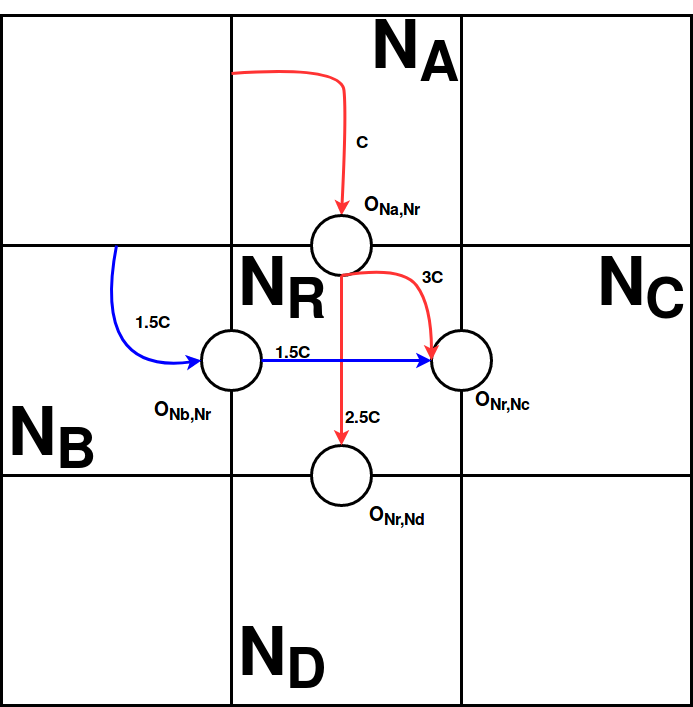
\includegraphics[width=0.6\textwidth]{LookaheadProblem}
\caption{A visual reference for the explanation of the lookahead problem in section 4.3}
\label{LookaheadRef}
\end{figure}

\section{Multi-Agent}
In a warehouse style environment, many things are being moved throughout the facility at any given time. If only a single robot were available to automate this process, it would be a highly ineffective system. Either that robot performs all tasks, creating a slow serial system, or humans still perform the majority of tasks, creating a hardly autonomous system. Therefore, it is necessary to have some arbitrary number of robots performing tasks in parallel for the system to be effective.
\subsection{Method}
Unfortunately, I do not have a warehouse scale facility to build and test this system in. Given that, the only way to implement and test what would be a multi-agent system is to use a multithreaded implementation.

In this implementation, each thread would be considered a path requested by a robot. Each thread has its own instance of data relating to the path being calculated. This includes cost, node parents, start location, end location, etc. 

In an attempt to stay true to the system, only one instance of the graph is used. This means that every thread will be accessing the "true" ceiling node rather than a copy of it. It also means the environment will be akin to a shared memory system. Because of this, any time a thread accesses a camera for information, it will need to ensure that the data on the relevant portions of the system are of its instance. This requires the use of locks in these situations. Aside from the addition of locks, the only change to D-A* is setting node information using local instance values, and setting local instance values using calculations performed on nodes.


Initially, I was setting the value of every node in the graph to the local instance values. As expected, this is horribly inefficient. It then occurred to me that the only nodes needing to be set are those in the open set. This is because the only nodes the algorithm is interested in are those on the open set. Any node on the closed set has already set its final values to the local instance. Any node not contained in a set has not yet been discovered and is therefore irrelevant. The only nodes being modified and used are those on the open set. However, it is necessary to set all nodes on the closed set with local instance values before rebuilding the path. If this is not done, the path information will be invalid. 

This change greatly increased the speedup as superfluous operations were removed. With that, I present the modifications to D-A* to allow multithreading in Algorithm \ref{MTD-A*}. As the open set and priority queue contain the same nodes and used similarly, I have not differentiated between the two up to this point. However, in this implementation, there is one portion where it is important to specify the distinction. Therefore, I have added one line where the priority queue and open set are handled in a very specific order.


\begin{algorithm}
\caption{MultiThreaded D-A*}
\label{MTD-A*}
\begin{algorithmic}[1]
\REQUIRE \ \\
Start Camera, $C_S$ \\
Goal Camera, $C_G$ \\
Start Point $P_S$ in $C_S$
\STATE set instance values for $C_S$
\STATE add $C_S$ to \textit{openSet}
\WHILE{\textit{openSet} is not empty}
	\STATE lock.acquire
	\STATE setNodes(\textit{openset})
	\STATE \textit{$N_C$} = \textit{openSet.pop}
	\STATE lock.release
	\IF{\textit{$N_C$} is $C_G$}
		\STATE add $N_C$ to \textit{closedset}
		\STATE lock.acquire
		\STATE setNodes(\textit{closedset})
		\RETURN $C_S$.rebuild\_path()
		\STATE lock.release
	\ENDIF
	\STATE let \textit{neighbors} be an initially empty list
\FOR{each \textit{neighbor} of \textit{$N_C$}}
	\IF{\textit{neighbor} in \textit{closedSet}}
		\STATE \textbf{continue}
	\ENDIF
	\IF{\textit{neighbor} not in \textit{openSet}}
		\STATE add \textit{neighbor} to \textit{openSet}
		\STATE lock.acquire
		\STATE setNodes(\textit{openset})
		\STATE add neighbor to priority queue
		\STATE lock.release
	\ENDIF
	\STATE add \textit{neighbor} to \textit{neighbors}
\ENDFOR	
\STATE lock.acquire
\STATE setNodes(openset)	 
\STATE $C_S$.getNeighborInfo(\textit{neighbors}, $N_C$, $C_G$)
\STATE setLocalInstanceValues(\textit{neighbors})
\STATE lock.release
\STATE \textit{closedSet}.add(\textit{$N_C$})
\STATE \textit{openSet}.remove(\textit{$N_C$})
\ENDWHILE
\RETURN failure
\end{algorithmic}
\end{algorithm}

\subsection{Issues}
This implementation was done in Python which comes with one main problem in regards to this system. When using a priority queue, any operation on the queue will resort the queue. By doing this, a problem is created in this system in that the nodes on each thread's queue are the "true" nodes rather than a local copy. If a thread updates a value on some node, then the next queue operation of a different thread whose queue contains that node will invalidate the queue.

Assume we have two threads, $A$ and $B$. Assume we have three nodes, $N_1, N_2,$ and $N_3$, whose costs are $7, 3,$ and $1$ respectively on thread $A$. If all of these nodes are inserted onto $A$'s queue, they will be in the order ${N_3, N_2, N_1}$. Suppose $B$ the cost of $N_1$ for $B$ is $2$. The cost value of $N_1$ will updated to $2$ and inserted into $B$'s queue. Upon doing this, the nodes will be in the order ${N_3, N_1, N_2}$ for $B$. At this point in time, $A$'s queue is still intact as no operations have been performed. Suppose $A$ then performs a GET call on the queue. Even though $N_1$ was inserted into $A$'s queue with a cost of $7$, the cost on $N_1$ is currently $2$ after $B$'s update. Therefore, after the GET call on $A$'s queue, the order will now be ${N_1, N_2}$. 

This problem causes a severe slowdown because there is a now a requirement to reinitialize the instance values of a thread onto all relevant nodes any time a queue operation is required. It is equivalent to a context switch on a processor. Due to the nature of A*, queue operations happen often which leads to several "context switches". Since each switch is a slow process, it is actually slower to allow every thread to attempt a path at once rather than in serial.The ability of the system to operate as multi-agent is not affected as several robots can still be given paths to be traversed simultaneously. It is, however, more efficient to calculate the paths one after another rather than in parallel.
\section{Results}
All results were simulated in Python using the networkx graph library. Simulation was performed on Ubuntu 16.04 using an i7 quad core processor.

All results in the pathing section were simulated on a variety of graphs. Parent grid sizes of 5x5, 10x10, 20x20, 50x50, and 100x100 were used. The rates of connectivity used on the child layer were 25\%, 50\%, and 75\%. Every permutation of grid size and connectivity rate were used giving a total of 15 total test cases. In each case a random graph was generated using a connectivity rate of 80\% on the parent layer. The child layer for each parent was given a random number of child nodes from 5 to 10. 1000 paths were run with each permutation giving a total of 15000 paths run each for Greedy, D-A* V1, and D-A* V2. This section compares the requests made and runtime of the two versions of D-A*. The cost is not compared as the cost is equal between the two methods as expected. The results of D-A* V2 are then compared to Greedy. In this case, cost is considered. D-A* V1 is not used in this comparison as V2 is nearly a complete improvement over V1.

For Multi-Agent testing, the same conditions apply. However, the 100x100 grid was omitted and only 100 paths were run for each permutation. This section will compare the times required to run paths serially vs in parallel using the multithreading method described in 5.1. Only D-A* V2 was used in this test. Since the goal of these results is to only compare runtime between the serial and multithreaded version of the same algorithm, only the most effective algorithm was tested.


I believe this grid size is a valid representation of the potential real system. Based on the assumption that a camera can see a 10x10 foot region from the ceiling of a warehouse with 1 foot of overlap, the viewable region is over 800,000 ft$^2$.

This section is going to focus on the real value results to show how the values scale with grid size and connectivity rate. Figures showing normalized value comparisons will be added into the Appendix.

\subsection{Pathing}
	\subsubsection{D-A* Comparison}
	In Figures \ref{fig:DAScompare25}, \ref{fig:DAScompare50}, and \ref{fig:DAScompare75}, the request count and runtime D-A* V1 and V2 are compared for all grid sizes with a connectivity rate of 25\%, 50\%, and 75\% respectively.
	
	As shown in the figures, the connectivity of the graph does not have much of an effect on the relative values of the two versions. While they do differ slightly, it's insignificant. The significance of these results lies in the comparison between the two versions at any connectivity. 
	
	At each grid size, the requests made by V2 is about 60\% of V1. It can also be seen that the runtime difference between the two versions is extremely small. The most significant difference sits at grid size 100 whose difference is slightly over 0.01 seconds on average. It should be noted that in this simulation, a request was not run through a network as I had no physical system. Requests were simulated by forcing the node being requested to call the corresponding function. Therefore, it is possible that the substantial difference in network requests will cause V1 to be slower than V2 in a real environment. Even if the request time of any average request is low enough to maintain a shorter runtime, the rate of requests may delay responses enough to tip runtime to the favor of V2.	
	
	It was mentioned in 4.2.2 that 66\% request reduction could not be achieved. Requests are made in other portions of the implementation, such as rebuilding the path, which are unaffected by the change made in V2. 
		\input{resultsfigs/real/DAStarComp25.tex}
		\input{resultsfigs/real/DAStarComp50.tex}
		\input{resultsfigs/real/DAStarComp75.tex}
	\subsubsection{D-A* vs Greedy}
	
	Due to the scale of difference between values generated by Greedy and D-A*, this section will focus on normalized results. In these results, D-A* values have been normalized to Greedy. Therefore, Greedy values are not represented on the charts as they are always one. Figures \ref{fig:DAGreedyPathLength}, \ref{fig:DAGreedyRequests}, and \ref{fig:DAGreedyRuntime} show the comparison between path length, request count, and runtime respectively.
	
	The results show that D-A* takes magnitudes longer to run than Greedy. This is expected as Greedy goes directly for the goal with no checks. It has neither the processing nor spread on the grid of D-A*, so it is expected that it runs much faster. For the same reason, the number of requests made by D-A* is up to 27 times the requests made by Greedy.
	
	Path length is fairly consistent across grid sizes. It does have a slight decline and reaches under 0.8 in one instance. 
	
	As stated in section 4.2.1, greedy sometimes outperforms D-A* in terms of path length. Out of the 15000 total paths generated, Greedy had a lower cost in 364 paths for a total of 2.42\%. While this number is very small, it is important to know what the average difference was. In Figure \ref{fig:GreedyOutperform}, the average path length of D-A* paths which were longer than Greedy are shown normalized to Greedy's path length. Based on the figure, there seems to be a slight downward trend for low and high connectivity as grid size increases. In the worst case, D-A* was 6.8\% longer; in the best case, 1.7\% longer. As the size of the area increases, this difference becomes more substantial in regard to real path length. Because the runtime of Greedy is magnitudes lower than D-A*, it would be possible to run both methods and take the shorter path.
	
	It should be noted that the "total" memory used in this system is higher than performing A* across the bottom layer as if each region were connected to its neighbors. Determining which path to take across a region requires knowing which of the available paths are the shortest; It is necessary to run a shortest path algorithm to determine this. 
	
In a static system, the paths through each node can be cached with much higher practicality than the paths across the entire child layer. Therefore, it is likely that this method would still outperform a non-hierarchical implementation in terms of memory used at runtime. 

However, in dynamic environment, especially one in which path costs are constantly changing, calculation of cost requires running a shortest path algorithm on the child layer. In this case, we are effectively pathing across the entire child layer as if it is not hierarchical. Due to the hierarchical nature of the implementation, there are some nodes that would be left unexpanded. The goal being found and verified as most optimal could leave some parent nodes unexpanded whose children would otherwise be expanded in a non-hierarchical implementation. However as this would not be the majority of the graph, we are still using more memory by pathing across both layers. If this system were centralized, this would be a real problem. 

However, the decentralized nature of this system renders the problem moot. This system has no concept of "total memory" as each node is a separate entity acting independently of the rest of the network. While the "total memory" used is higher, the memory used on any given node is much lower. The source node uses the most memory by pathing across its child layer while also managing the queue and sets required to path across the parent layer. With the decentralized implementation, the number of nodes expanded in the parent layer is equal to the centralized implementation. Therefore, we can ignore the parent layer in this memory comparison.

With the disregard of the parent layer, the memory of the centralized system becomes the entirety of the expanded set of nodes on the child layer. The memory of the decentralized system is then divided into the individual nodes used. As each node only handles a small subset of points on the child layer, the memory of a single node in this graph is greatly reduced to about $\frac{C}{N}$ where $N$ is the number of expanded nodes in the parent layer and $C$ is the number of nodes expanded in the child layer. Thereofre, I claim that this increase in total memory is not a true problem in this system.

	\input{resultsfigs/normalized/DAGreedyRuntime.tex}
	\input{resultsfigs/normalized/GreedyOutperform.tex}
\subsection{Multi-Agent}
Multi-Agent did not pan out as initially expected. The run time with multithreading is worse than running in serial. The reason for this is described in Section 5.2. 

The runtime comparison results are shown in Figure \ref{fig:MTCompare}. Looking at the figure, it can be seen that the runtime of the multithreaded implementation climbs quickly as the size of the grid grows. This rapid growth is the reason grid size 100 is not represented in these results. The reason why this happens was discussed in Section 5.2.

Methods of potentially improving the runtime of the multithreaded implementation are discussed in Section 7.2.

\input{resultsfigs/real/MT.tex}
\input{futurework.tex}
\section{Conclusion}
In this work, I defined and implemented the base for a system which would allow multi-agent decentralized path planning through a static or dynamic area. As intended, this is the base navigation system on which any number of specific tasks could be implemented using various robots. Areas in which this method is superior to existing methods were discussed.

I presented results obtained via simulation showing that this type of system design is possible. I discussed multiple problems with this implementation and ways they can potentially be fixed or mitigated in future work.

Two different versions of D-A* were compared to show improvement over the original. This implementation allows an entire path to be calculated at once rather than regenerating a path upon entering a new region as several referenced works did. This saves time by reducing how many paths are generated through a region by a single robot, and, in the case of only pathing through one camera at a time, outperforms a greedy-based search over 97\% of the time.

Unfortunately I was not able to put together an implementation of deadlock for this project. In lieu of this, I presented ideas used in other works and explained why I believe they could be effective deadlock prevention in this system.
\section{Acknowledgements}
This work was supported in part by the national science foundation (NSF) under Grant 1547934.


\bibliographystyle{IEEEtran}
\begin{thebibliography}{60} % FIXME update this number to the amount of references used %

\bibitem{DeadlockDigani}
V.~Digani, L.~Sabattini, C.~Secchi, and C.~Fantuzzi. "Hierarchical  Traffic Control for Partially Decentralized Coordination of Multi AGV Systems in Industrial Environments." \emph{Proceedings of the IEEE International Conference On Robotics \& Automation (ICRA), 2014}., pp.6144-6149.

\bibitem{DeadlockJager}
M.~Jager and B.~Nebel. "Decentralized collision avoidance, deadlock detection, and deadlock resolution for multiple mobile robots." \emph{Proceedings of the IEEE/RSJ International Conference on Intelligent Robots and Systems, 2001}., vol. 3, 2001, pp. 1213-1219 vol.3.

\bibitem{DeadlockDraganjac}
I.~Draganjac, D.~Mikli{\'c}, Z.~Kova{\v c}i{\'c}, G.~Vasiljevi{'c}, S.~Bogdan. "Decentralized Control of Multi-AGV Systems in Autonomous Warehousing Applications." \emph{Proceedings of the IEEE Transactions on Automation Science and Engineering, 2016}., vol. 13, no. 4, pp. 1433-1447.

\bibitem{WaypointJia}
D.~Jia, C.~Hu, K.~Qin, and X.Cui. "Planar Waypoint Generation and Path Finding in Dynamic Environment." \emph{Proceedings of the International Conference on Identification, Information, and Knowledge in the Internet of Things, 2014}., pp. 206-211.

\bibitem{LaValleAlgorithms}
J.~Yu and S.~LaValle. "Optimal Multi-Robot Path Planning on Graphs: Complete Algorithms and Effective Heuristics." CoRR, abs/1507.03290, July 2015.

\bibitem{FTC-A}
C.~Zhong, S.~Liu, B.~Zhang, Q.~Lu, J.~Wang, Q.~Wu, and F.~Gao. "A Fast On-line Global Path Planning Algorithm Based on Regionalized Roadmap for Robot Navigation." IFAC-PapersOnLine, vol. 50, issue 1, pp. 319-324, July 2017.

\bibitem{DecentralizedPlanningVelagapudi}
P.~Velagapudi, K.~Sycara, and P.~Scerri. "Decentralized prioritized planning in large multirobot teams." \emph{2010 IEEE/RSJ International Conference on Intelligent Robots and Systems, 2010}., pp. 4603-4609.

\bibitem{PlanningSurveyParker}
L.E.~Parker. "Path Planning and Motion Coordination in Multiple Mobile Robot Teams." \emph{Encyclopedia of complexity and system science, 2009}., pp. 5783-5800.

%\bibitem{MeanShiftComaniciu}
%D.~Comaniciu, and P.~Meer. "Mean Shift: A Robust Approach Toward Feature Space Analysis." \emph{IEEE Transactions on pattern analysis and machine intelligence}., vol. 24, no. 5, May 2002.

\bibitem{WaypointVideoGames}
X.~Cui, and H.~Shi. "A*-based pathfinding in modern computer games." \emph{International Journal of Computer Science and Network Security}., vol. 11, no. 1, pp. 125-130, 2011.

\bibitem{CTF-A}
J.Y.~Lee, and W.~Yu. "A Coarse-to-Fine Approach for Fast Path Finding for Mobile Robots." \emph{Proceedings from IEEE/RSJ International Conference on Intelligent Robots and Systems, 2009}., pp. 5414-5419. 

%\bibitem{FranzMS}
%F.J.~Streit, M.J.H.~Pantho, C.~Bobda, C.~Roullet. "Vision-Based Path Construction and Maintenance for Indoor Guidance of Autonomous Ground Vehicles Based on Collaborative Smart Cameras." \emph{Proceedings of the 10th International Conference on Distributed Smart Camera, 2016}., pp. 44-49.

\bibitem{SLAM}
M.G.~Dissanayake, P.~Newman, S.~Clark, H.F.~Durrant-Whyte, and M.~Csorba. "A solution to the simultaneous localization and map building (SLAM) problem." \emph{IEEE Transactions on robotics and automation, 2001}., vol. 17, no. 3, pp.229-241.

\bibitem{DecentralizedSLAM}
K.Y.K.~Leung, T.D.~Barfoot, H.H.T.~Liu. "Distributed and Decentralized Cooperative Simultaneous Localization and Mapping for Dynamic and Sparse Robot Networks."\emph{Proceedings of the IEEE International Conference on Robotics and Automation, 2011}., pp. 3841-3847.

\bibitem{HPA}
A.~Botea, M.~Muller, J.~Schaeffer. "Near Optimal Hierarchical Path-Finding." \emph{Journal of Game Development, 2004}., pp. 7-28

\bibitem{HierarchicalA}
R.C.~Holte, M.B.~Perez, R.M.~Zimmer, A.J.~MacDonald. "Hierarchical A*: Searching Abstraction Hierarchies Efficiently." \emph{Proceedings of the Thirteenth national Conference on Articical Intelligence, 1996}., vol. 1, pp. 530-535.
\end{thebibliography}

\newpage

\input{appendix.tex}

\end{document}